%!TEX root = ../report.tex
\documentclass[../report.tex]{subfiles}
\begin{document}
    \chapter{Solution}
    \section{GestaltMatcher Architecture}
    The procedure to diagnose rare-genetic syndromes from patient faces using GestaltMatcher is described in a detailed manner in Chapter 2 \ref{}. This section describes the architecture of its underlying Convolutional Neural Network (CNN) backbone and steps involved in preprocessing its input images. The pipeline shown in \ref{} Figure illustrates the sequence of steps involved in processing a patient photo using GestaltMatcher.
    \begin{figure}[ht]
     \hspace*{1.0cm}      
     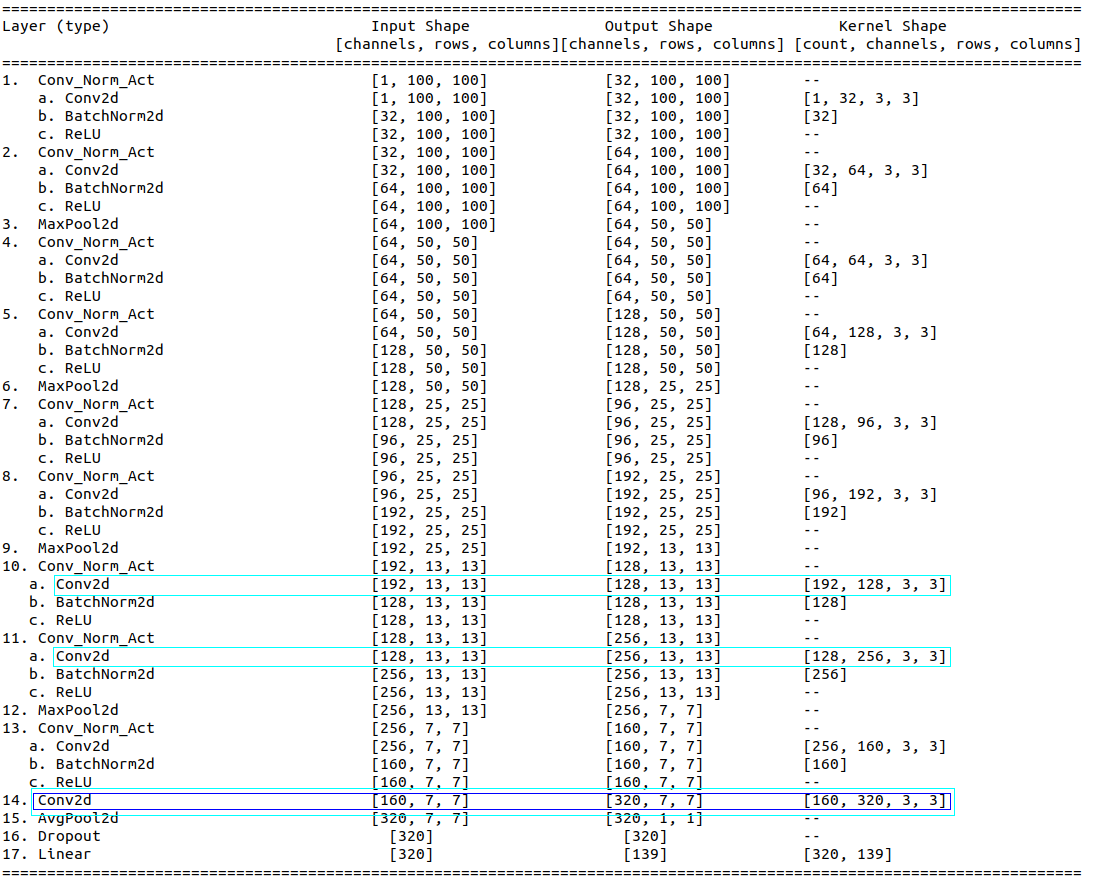
\includegraphics[scale=0.4]{chapter5/gestalt_matcher_arch.png}
     \caption{Architecture of the CNN in GestaltMatcher. The convolution layer (Layer. 14) used to generate attribution maps using GradCAM and HiResCAM methods
     is highlighted using a blue box. Layers (Layer 10.a, Layer 11.a and Layer.14) that are used by the CustomGradCAM method are highlighted using cyan boxes. }
     \label{fig_arch_gest_matcher}
    \end{figure}
    \section{Explanation Methods - GestaltMatcher Integration}
    \section{Experiments}
    \subsection{Patient-wise Attribution Map Generation}
    \subsection{Composite Face Generation}
    \subsection{Syndrome-wise Attribution Map Generation}
    \subsection{Dataset Imbalance - Explanation Quality Analysis}
\end{document}
